%-------------------------------------------------------------------------------
% File: modelling.tex
%       Epidemic Broadcast project documentation.
%
% Author: Marco Pinna, Rambod Rahmani, Yuri Mazzuoli
%         Created on 05/12/2020
%-------------------------------------------------------------------------------
\chapter{System modelling}
\label{ch:modelling}
Wireless communication networks have been extensively studied in scientific
literature and one of the most used mathematical tools to model them and their
behaviour is \textit{graph theory}. In this work the same approach was used.\\
As the broadcast progresses and the message is transmitted among the nodes, the system evolves through different states where each node could be listening for an incoming message, transmitting it, or could have already sent the message and stopped.\\
The different nodes behaviours were modelled by means
of three different states:
\begin{itemize}
	\item \texttt{listening}: the node has not received the broadcast message
	yet and therefore it is still listening for incoming messages from other nodes;
	\item \texttt{transmitting}: the node has received the message and during
	each time slot it is trying to transmit it to adjacent nodes; in what
	follows, \texttt{transmitting} nodes will also be referred to as
	\textit{active} nodes;
	\item \texttt{sleeping}: the node has already received and retransmitted
	the broadcast message; once a node enters the \texttt{sleeping} state, it
	remains in such state and will therefore have no effect on the system
	any more.
\end{itemize}
\section{Graph model for wireless systems}\label{sec:graphModelForWirelessSystems}
The $N$ users dropped on the floorplan make up the set of vertices $V$ of a
graph $G$, whose set of edges $E$ is composed by all the connections between
pairs of nodes in reach of each other. Consider the following as a simplified
scenario to exemplify this model: in figure \ref{fig:graph1} (a) devices A, C
and D are within device B transmission radius. In the equivalent graph, there
will be edges that connect B to A, to C and to D. The same goes for all the
other vertices. The resulting graph is shown in figure \ref{fig:graph1} (b).
\begin{figure}[H]
	\begin{minipage}{.5\textwidth}
        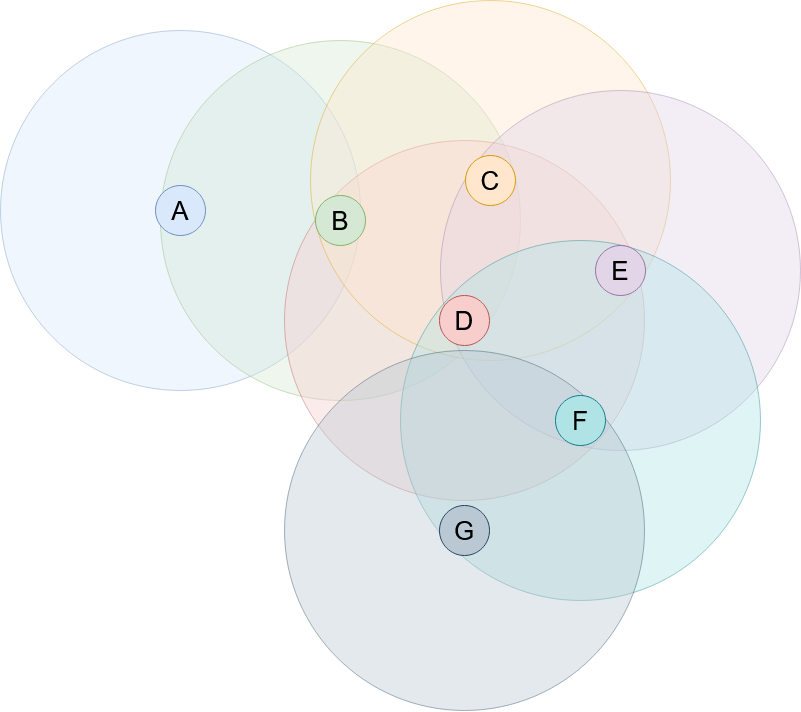
\includegraphics[scale=.23]{img/wireless_graph_1.png}
        \begin{center}
            a) Ranges representation
        \end{center}
	\end{minipage}
	\begin{minipage}{.5\textwidth} 
		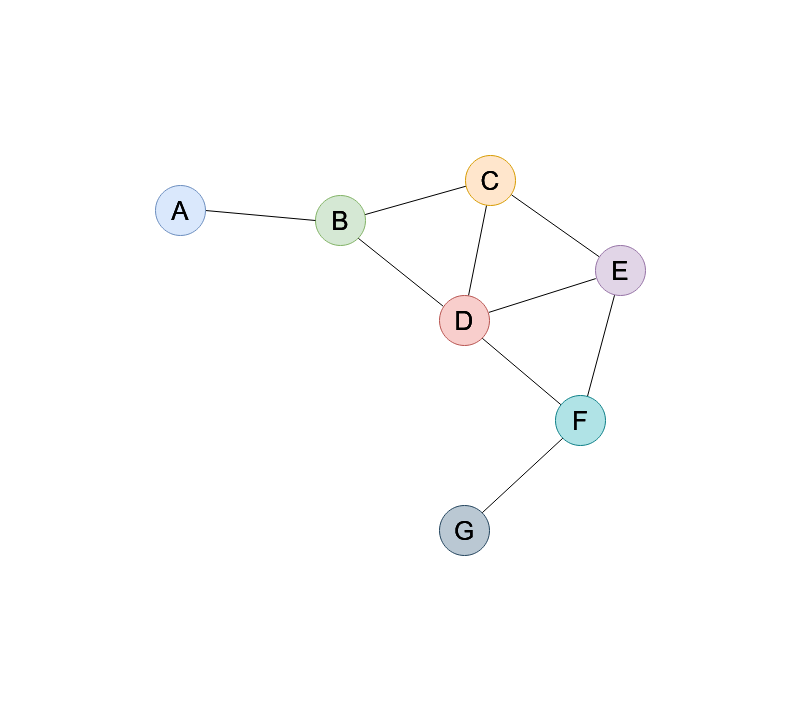
\includegraphics[scale=.23]{img/wireless_graph_2.png}
		\begin{center}
            b) Equivalent graph representation
        \end{center}
	\end{minipage}
	\caption{}
    \label{fig:graph1}
\end{figure}
\noindent
In general, the existence of an edge from vertex $i$ to vertex $j$ means that
nodes $i$ and $j$ are within reach of each other. Two vertices connected by an
edge are said to be \textit{adjacent}. The set composed by all the vertices adjacent to a vertex $v$ is called the
\textit{neighbourhood of v}.\\
During the broadcast process, a node can only receive
from and transmit to its neighbourhood.\\
Once a node has transmitted the message and has gone into the \texttt{sleeping}
state, from the point of view of the graph model, it disappears, along with all
the edges connected to it. Therefore, the set of vertices $V$ changes with time.
This is what in literature is called a \textit{dynamic graph} or, more
%TODO fix citation
specifically, a \textit{node-dynamic graph} [\cite{hararygraph}].\\

Modelling the system with graphs also allows for the simple computation of some of their properties, such as the \textit{eccentricity}; in this way, it is possible to find theoretical lower bounds for some of the metrics and can also be useful for validating the simulator or for gaining further insight about the results.\\
Given a graph $G(V, E)$ which represents the users
in the floorplan, let node $v^{*}$ be the starting point for the broadcast, i.e.
the first node with the message. In the best case scenario, the system evolves
with no collisions at all and the message moves along the paths of the graph,
reaching all nodes. Let $d(u, v)$ be the \textit{distance} between two vertices
$u$ and $v$, i.e. the length of the shortest directed path from $u$ to $v$
consisting of arcs, provided at least one such path exists. Then, the lower
bound for the broadcast time is given by the highest distance between $v^{*}$
and any other vertex. This quantity, in graph theory, is called
\textit{eccentricity} of the vertex $v^{*}$. More formally, the eccentricity of
$v^{*}$ is defined as follows:
\begin{equation}
\epsilon(v^{*}) = \max_{u{\in}V} d(v^{*}, u)
\end{equation}
Another observation to be made is that the existence of an edge between two nodes only depends on the ratio between their radius and their distance. This implies that 100 nodes with a radius of 15 m dropped in a 100 m x 100 m floorplan will produce the exact same graph as 100 nodes having a radius of 1,5 m dropped in a 10 m x 10 m floorplan, if all their coordinates are just scaled by a factor of 10.\\ 
\section{Simplified models}
In what follows, incrementally more complex scenarios are presented showing the
reasoning that led us to obtain the final complete model.
\subsection{Single queue configuration}\label{ssec:singlequeue}
Let us consider a configuration where users are arranged in a line, as shown in
figure \ref{fig:single_queue_graph}. Each user only has two neighbours, except for
the outer ones (nodes $A$ and $E$) that only have one. Assuming node $A$ is the
starting user with the broadcast message, it is the only node in
\texttt{transmitting} state while all the other nodes are initially in
\texttt{listening} state. 
\begin{figure}[H]
    \begin{center}
        
\includegraphics[scale=0.6]{img/single_queue.png}
        \caption{Graph of the Single queue configuration}
        \label{fig:single_queue_graph}
    \end{center}
    \vspace*{-0.4cm}
\end{figure}
\noindent It is clear that, with this configuration, each listening node has a
maximum of one active node in its neighbourhood at any time and thus cannot possibly receive
the message from two different sources at the same time. This guarantees the
absence of collisions.\\
In such a scenario, $100\%$ asymptotic coverage is
ensured: during each slot, the active node extracts a Bernoullian RV with
success probability $p$. The probability of the active node transmitting after exactly
$k$ slots is a geometric distribution:
\begin{equation}
	P(X = k) = (1 - p)^{k-1} \cdot p
	\label{geometricDistribution}
\end{equation}
The successful transmission of the message from an active node to its neighbour
is thus guaranteed since $\lim_{k \to \infty} (1 - p)^{k-1} \cdot p = 0$.
As for the total broadcast time \texttt{T}, on average it is equal to the mean
value of the geometric distribution, $\frac{1}{p}$, times the number of hops
needed to reach the last node:
\begin{equation}
	E[T] = \frac{1}{p} \cdot (N - 1).
	\label{eq:singleQueueMeanT}
\end{equation}

\subsection{Star configuration with one active node (star 1-to-5)}
\label{ssec:star1}
Another useful simple configuration worth analysing is the star-shaped one. In
this setup, there is a central node $A$ connected to $N - 1$ nodes, all of which
are non-adjacent to each other. Let us suppose $A$ to be the broadcast starter.
The absence of collisions is ensured in this scenario as well, for the
same reason as the previous configuration.
At each time slot, $A$ extracts a Bernoulli RV. When the extraction is
successful, $A$ broadcasts the message its entire neighbourhood and total
coverage is reached. Hence, 100\% asymptotic coverage is ensured in this case
too, as the probability of $A$ not transmitting for $k$ consecutive slots is
given by Eq. \ref{geometricDistribution} and goes to $0$ as $k$ goes to
infinity.
\begin{figure}[H]
    \begin{center}
        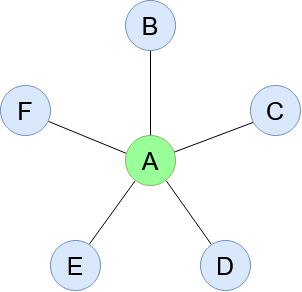
\includegraphics[scale=0.4]{img/star_graph.png}
        \caption{Graph of the star configuration with one active node}
        \label{fig:star1to5}
    \end{center}
\end{figure}
\noindent
In this case, the average total broadcast time $E[T]$ is simply equal to the
mean value of the geometric distribution, $\frac{1}{p}$, since the central
node is placed at one hop of distance from all the remaining nodes.\\
\\
If the broadcast starter node was not the one placed in the center of the star,
there would not be much difference: absence of collisions and total coverage
would be ensured as well. As far as it concerns the total broadcast time
\texttt{T}, its expected value would just be $\frac{2}{p}$, since
the are now \textbf{two} hops involved in the broadcast: one from the starter
node to the center node and the another from the center node to all the $N - 2$
remaining ones.

\subsection{Star configuration with all nodes active but one (star 5-to-1)}
\label{ssec:star2}
\begin{figure}[H]
    \begin{center}
        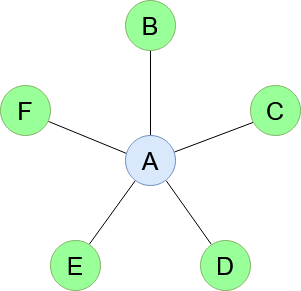
\includegraphics[scale=0.4]{img/star_graph2.png}
        \caption{Graph of the star configuration with all nodes active but one}
        \label{fig:star5to1}
    \end{center}
\end{figure}
This configuration can be seen as the complement of the previous one: all the nodes
on the rays of the star are active and trying to transmit the message to the
center node. This is the first scenario where collisions might occur and with a non-zero probability that
total coverage might never be reached. To simplify the
analysis of this system and obtain some insights, it is useful to model it by
means of a discrete-time Markov chain.
\subsubsection{Discrete-time Markov chain model for N nodes transmitting to a target}
Since the state of the system evolves only once per slot, it can be modelled
with a discrete-time Markov chain (DTMC) as follows:
\begin{figure}[H]
    \begin{center}
        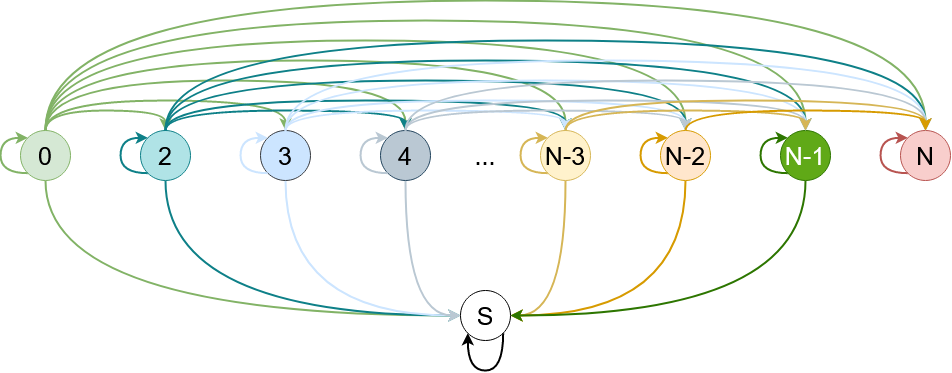
\includegraphics[scale=0.4]{img/DTMC.png}
        \caption{Discrete-time Markov chain for a scenario with N active devices}
        \label{fig:dtmc}
    \end{center}
\end{figure}
\noindent Figure \ref{fig:dtmc} shows the DTMC for a generic configuration with
$N$ transmitters (transition probabilities are not shown for the sake of clarity).\\
State $0$ and states $2$ to $N$ represent the number of \texttt{sleeping}
devices, namely devices that have already sent the message and have stopped. The
number of \texttt{sleeping} devices was chosen over the number of
\texttt{transmitting} devices as the former only allows for non-decreasing
sequences of states, since a device cannot become active again once it enters
the \texttt{sleeping} state.\\
State $S$ represents the successful transmission state, which the system
transitions to when only one device has transmitted the message during the
previous time slot.\\
The initial state $X_{0}$ is $0$. Any transition from a state $i$ to a state
$j$, $j \neq S$, means that more than one device has transmitted the message, 
resulting in the target device detecting a collision.
Both state $S$ and state $N$ are \textit{absorbing states}, i.e. states that,
once entered, cannot be left (as can be seen in Figure \ref{fig:dtmc}, where the
only outgoing arrow from these states goes back to the state itself).\\
If the system transitions to state $N$, it stays in it indefinitely since all
the devices are \texttt{sleeping} and they cannot become active again. This
implies that there will never be total coverage since the target device will
forever stay in the \texttt{listening} state without ever receiving the message.
On the other hand, state $S$, despite being an absorbing state as well, should
actually be considered as an ``exit" state rather than a ``sink" state: if the
system transitions to this state, the target device has successfully received
the message and total coverage has been reached.\\
Another interesting observation concerns state $N - 1$: if the system reaches
this state, as there is one and only one remaining node which can transmit, it
is guaranteed that the target device will sooner or later receive the message,
for the same reason set forth in \ref{ssec:singlequeue}.
\subsubsection{Transition probabilities}
Let us now address the challenging part: computing the transition probability.\\
During the first slot, the probability that $j$ devices out of $N$ transmit
the message is given by:
\begin{equation}
    P_{1}(j, N) = {N \choose j} p^{j} (1 - p)^{N - j}
    \label{eq:firstSlotTransProb}
\end{equation}
\hfill \break
which is a binomial distribution given by the sum of the N Bernoulli distributions.\\
\\
As for the probability of $j$ devices transmitting at the same time during slot
$k$, be it $P_{k}(j)$, we can model the system as if it was in the first slot,
with the total number of active devices now being equal to $N$ - $t$, where $t$
is the total number of devices that have transmitted up to the $(k\text{-}1)$-th
time slot.\\
Carrying on with the computation of the transition probabilities this way, leads
to unsatisfactory results which are difficult to interpret.\\
\\
A better way to compute the probability of having $j$ devices sleeping at
slot $k$, is to use the \textit{stochastic matrix} of the Markov chain. If the
probability of moving from state $i$ to $j$ in one time slot is
$Pr(j|i) = P_{i,j}$, the stochastic matrix $P$ is given by using
$P_{i,j}$ as the $i$-th row and $j$-th column element, e.g.
\begin{equation*}
P = 
\begin{bmatrix}
P_{0,0}	& P_{0,S}	& P_{0,2}	& \dots  	& P_{0,j}	& \dots		& P_{0,N} \\
P_{S,0}	& P_{S,S}	& P_{S,2}	& \dots  	& P_{S,j}	& \dots		& P_{S,N} \\
P_{2,0}	& P_{2,S}	& P_{2,2}	& \dots  	& P_{2,j}	& \dots		& P_{2,N} \\
\vdots	& \vdots	& \vdots	& \ddots 	& \vdots	& \ddots	& \vdots \\
P_{i,0}	& P_{i,S}	& P_{i,2}	& \dots		& P_{i,j}	& \dots		& P_{i,N} \\
\vdots	& \vdots	& \vdots	& \ddots	& \vdots	& \ddots	& \vdots \\
P_{N,0}	& P_{N,S}	& P_{N,2}	& \dots		& P_{N,j}	& \dots		& P_{N,N} \\
\end{bmatrix}
\label{stochasticMatrix1}
\end{equation*}
Since S and N are absorbing states, $P_{S,j}=0$ for j $\neq$ S and $P_{N,j} = 0$
for $j \neq N$.\\
Moreover, all the possible transitions can only generate a non-decreasing
sequence of states and there are no transitions between states that differ by
one, hence\\
$P_{i, j} = 0$ $\forall$ $i > j$ and $\forall$ $j = i + 1$.\\
All the other elements of the matrix can be computed using the following formula:
\begin{equation}
    P_{i,j} = {N-i\choose j - i} p^{j - i} (1-p)^{N - j}
    \label{eq:matrixElementProb}
\end{equation}
and $P_{i,S}$ is given by:
\begin{equation}
    P_{i,S} = {N-i\choose 1} p(1-p)^{N - i - 1}
    \label{eq:matrixProbToS}
\end{equation}
which is just a particular case of \eqref{eq:matrixElementProb} when $j = i + 1$.\\
Therefore the stochastic matrix becomes:
\begin{equation*}
P = 
\begin{bmatrix}
P_{0,0}	& P_{0,S}	& P_{0,2}	& \dots  	& P_{0,j}	& \dots		& P_{0,N} \\
0		& 1			& 0			& \dots  	& 0			& \dots		& 0		 \\
0		& P_{2,S}	& P_{2,2}	& \dots  	& P_{2,j}	& \dots		& P_{2,N} \\
\vdots	& \vdots	& \vdots	& \ddots 	& \vdots	& \ddots	& \vdots \\
0		& P_{i,S}	& 0			& \dots		& P_{i,j}	& \dots		& P_{i,N} \\
\vdots	& \vdots	& \vdots	& \ddots	& \vdots	& \ddots	& \vdots \\
0		& 0			& 0			& \dots  	& 0			& \dots		& 1		 \\
\end{bmatrix}
\label{stochasticMatrix2}
\end{equation*}
Let $x_{0}$ be the \textit{initial state vector}, i.e. an $N \times 1$ vector
that describes the probability distribution of starting at each of the $N$
possible states.\\
To compute the probability of transitioning to state $j$ in \textbf{k} steps, it
is now sufficient to multiply the initial state vector $x_{0}$ by the stochastic
matrix raised to the $k$-th power, e.g.
\begin{equation}\label{probAtStateK1}
P_{k}(j) = (x_{0}\cdot P^{k})_{j}
\end{equation}
In our case, the system always starts in state 0, so we have
\begin{equation*}
x_{0} = 
\begin{bmatrix}
1 \\
0 \\
0 \\
\vdots \\
0
\end{bmatrix}
\label{initialStateVector}
\end{equation*}
which yields
\begin{equation}
P_{k}(j) = 
\begin{bmatrix}
1 \\
0 \\
0 \\
\vdots \\
0
\end{bmatrix}
\cdot P^{k} = (P^{k})_{0,j}
\label{eq:PkOfJ}
\end{equation}
Calculating the $k$-th power of a matrix can be an intensive task from a
computational point of view. To improve the complexity of the computation, rows
and columns of P can be rearranged, moving the S row and the S column as
penultimate, thus obtaining
\begin{equation*}
P = 
\begin{bmatrix}
P_{0,0}	& P_{0,2}	& P_{0,3}  	& \dots	& P_{0, N-1}	& P_{0,S}	& P_{0,N} \\
		& P_{2,2}	& 0  	& \dots	& P_{2, N-1}	& P_{2,S}	& P_{2,N} \\
		& 			& P_{3,3}	& \dots	& P_{3, N-1}	& P_{3,S}	& P_{3,N} \\
 		& 			& 			& \ddots& \vdots		& \vdots	& \vdots \\
		& 			& 			& 		& P_{N-1,N-1}	& P_{N-1,S}	& 0\\
		& 			& 			& 		& 				& 1			& 0		 \\
0		& 			& 		  	& 		& 				& 			& 1		 \\
\end{bmatrix}
\label{triangularPMatrix}
\end{equation*}
$P$ is now an upper triangular matrix and this allows for faster computation of
its powers in \ref{eq:PkOfJ}.
